\documentclass[border=3pt,tikz]{standalone}
% Shared look for every TikZ figure in these notes.
% Included by each standalone figure file; also keeps the figures consistent
% with the colours used in the PDF and on the website.

\usepackage{tikz}
\usepackage{pgfplots}
\pgfplotsset{compat=1.18}
\usetikzlibrary{arrows.meta, decorations.markings, decorations.pathmorphing,
                patterns, calc, positioning}
\usepackage{amsmath}

% Series colours are the three validated categorical slots also used by the
% interactive widgets, so a path drawn in the printed notes and the same path on
% the website are the same colour. They clear the colour-vision-deficiency and
% contrast checks as a set; every path is direct-labelled as well, so colour is
% never the only thing carrying identity.
\definecolor{duPurple}{HTML}{68246D}
\definecolor{duBlue}{HTML}{2A78D6}
\definecolor{duRed}{HTML}{EB6834}
\definecolor{duGreen}{HTML}{1BAF7A}
\definecolor{duGrey}{HTML}{6B6B6B}

\tikzset{
  axisline/.style   = {-{Stealth[length=3mm]}, line width=0.7pt, black},
  path1/.style      = {duBlue,   line width=1.1pt},
  path2/.style      = {duRed,    line width=1.1pt},
  path3/.style      = {duGreen,  line width=1.1pt},
  statedot/.style   = {circle, fill=black, inner sep=1.4pt},
  arrowhead/.style  = {decoration={markings,
                        mark=at position #1 with {\arrow{Stealth[length=2.6mm]}}},
                       postaction={decorate}},
  lbl/.style        = {font=\small},
  slbl/.style       = {font=\footnotesize, duGrey},
  workfill/.style   = {duPurple, opacity=0.16},
}

% Carnot cycle on a T-s diagram
\begin{document}
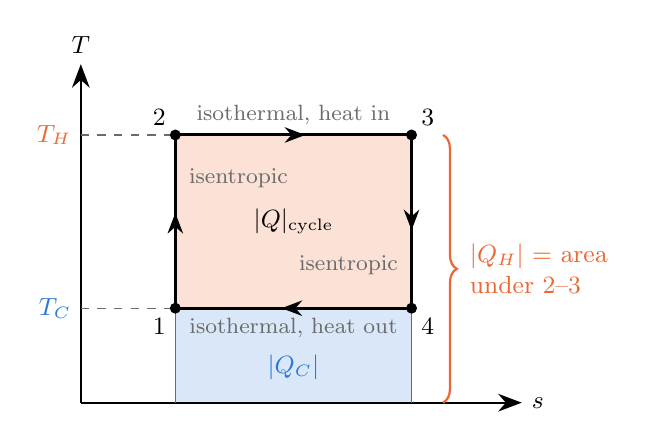
\begin{tikzpicture}[x=1cm,y=1cm]
  \fill[duBlue, opacity=0.18] (1.2,0) rectangle (4.2,1.2);
  \fill[duRed, opacity=0.20] (1.2,1.2) rectangle (4.2,3.4);
  \draw[axisline] (0,0) -- (5.6,0) node[right, lbl] {$s$};
  \draw[axisline] (0,0) -- (0,4.3) node[above, lbl] {$T$};
  \draw[line width=1.1pt, arrowhead=0.55] (1.2,1.2) -- (1.2,3.4);
  \draw[line width=1.1pt, arrowhead=0.55] (1.2,3.4) -- (4.2,3.4);
  \draw[line width=1.1pt, arrowhead=0.55] (4.2,3.4) -- (4.2,1.2);
  \draw[line width=1.1pt, arrowhead=0.55] (4.2,1.2) -- (1.2,1.2);
  \draw[duGrey, dashed] (0,3.4) node[left, lbl, duRed] {$T_H$} -- (1.2,3.4);
  \draw[duGrey, dashed] (0,1.2) node[left, lbl, duBlue] {$T_C$} -- (1.2,1.2);
  \draw[duGrey] (1.2,0) -- (1.2,1.2); \draw[duGrey] (4.2,0) -- (4.2,1.2);
  \foreach \p/\l/\a in {{(1.2,1.2)}/1/below left, {(1.2,3.4)}/2/above left, {(4.2,3.4)}/3/above right, {(4.2,1.2)}/4/below right}
    { \node[statedot] at \p {}; \node[lbl, \a] at \p {\l}; }
  \node[lbl] at (2.7,2.3) {$|Q|_\text{cycle}$};
  \node[lbl, duBlue] at (2.7,0.45) {$|Q_C|$};
  \draw[decorate, decoration={brace, amplitude=5pt}, duRed, line width=0.8pt] (4.6,3.4) -- (4.6,0) node[midway, right=6pt, lbl, align=left] {$|Q_H|$ = area\\ under 2--3};
  \node[slbl, above] at (2.7,3.4) {isothermal, heat in};
  \node[slbl, anchor=west] at (1.25,2.85) {isentropic};
  \node[slbl, anchor=east] at (4.15,1.75) {isentropic};
  \node[slbl, below] at (2.7,1.2) {isothermal, heat out};
\end{tikzpicture}
\end{document}
